\begin{center}
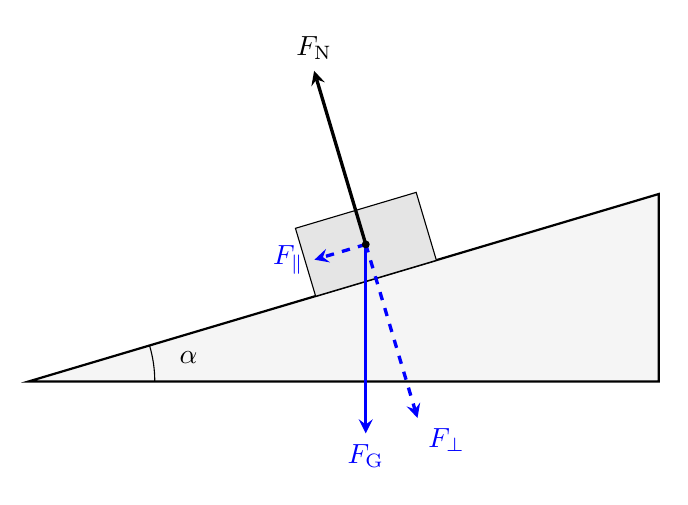
\begin{tikzpicture}[>=stealth]
 \draw[thick, fill=gray!8] (0,0) -- (8.00,0) -- (8.00,2.38) -- cycle;
 \draw (1.6,0) arc (0:16.58:1.6);
 \node at (2.03,0.30) {$\alpha$};
 \begin{scope}[shift={(4.41,1.31)}, rotate=16.58]
  \draw[fill=gray!20] (-0.8,0) rectangle (0.8,0.9);
 \end{scope}
 \draw[->, very thick, blue] (4.28,1.74) -- ++(-90.00:2.40) node[anchor=north] {$F_\mathrm{G}$};
 \draw[->, very thick, blue, dashed] (4.28,1.74) -- ++(-73.42:2.30) node[anchor=north west] {$F_\perp$};
 \draw[->, very thick, blue, dashed] (4.28,1.74) -- ++(196.58:0.68) node[anchor=east] {$F_\parallel$};
 \draw[->, very thick, black] (4.28,1.74) -- ++(106.58:2.30) node[anchor=south] {$F_\mathrm{N}$};
 \fill (4.28,1.74) circle (0.05);
\end{tikzpicture}
\end{center}

Ohne Reibung ist die Hangabtriebskraft $F_\parallel = m\,g\sin\alpha$ die resultierende Kraft. Aus $m\,a = m\,g\sin\alpha$ folgt $\sin\alpha = a/g$:
\begin{align}
 \alpha &= \wiF = \arcsin\left(\frac{\aEb}{\gE}\right) = \wi \approx \result{\wiP{0}{2}}
\end{align}
Die Normalkraft ist gleich der Komponente der Gewichtskraft senkrecht zur Ebene, $F_\mathrm{N} = m\,g\cos\alpha$. Ihre relative Abweichung von der Gewichtskraft ist
\begin{align}
 \frac{F_\mathrm{N}-F_\mathrm{G}}{F_\mathrm{G}} &= \frac{m\,g\cos\alpha - m\,g}{m\,g} = \devF \\
   &= \cos\left(\wi\right)-1 = \dev \approx \result{\devP{0}{2}}
\end{align}
